\section{Implementation}
\nopagebreak[4]
\subsection{Relational Model Overview}

After the conceptual design was finalized through the ER diagram, the next step was to convert that design into a relational schema suitable for implementation in a relational DBMS. The resulting schema was designed to preserve the structure of the conceptual model while supporting the application features required by Urban Scout.

The implementation includes relations for users, administrators, regions, places, specialized place types, transit services, transit routes, news posts, safety alerts, incident reports, itineraries, and associative relationships connecting those entities. The schema reflects the standard transformation process from entity-relationship design to a relational model. Strong entities became base relations, specialization was implemented through subtype tables, weak entities were converted using composite keys, and many-to-many relationships were represented through linking tables.

The final relational structure supports both the frontend interface and backend endpoints. Each table has a clear role in storing core data or representing relationships between entities, which allows the system to retrieve connected information efficiently. The relational schema and UML class diagrams (Figures~\ref{fig:rm} and~\ref{fig:uml}) illustrate the full set of tables and their relationships.

\begin{figure}[p]
    \centering
    \IfFileExists{figures/relational-model.png}{%
        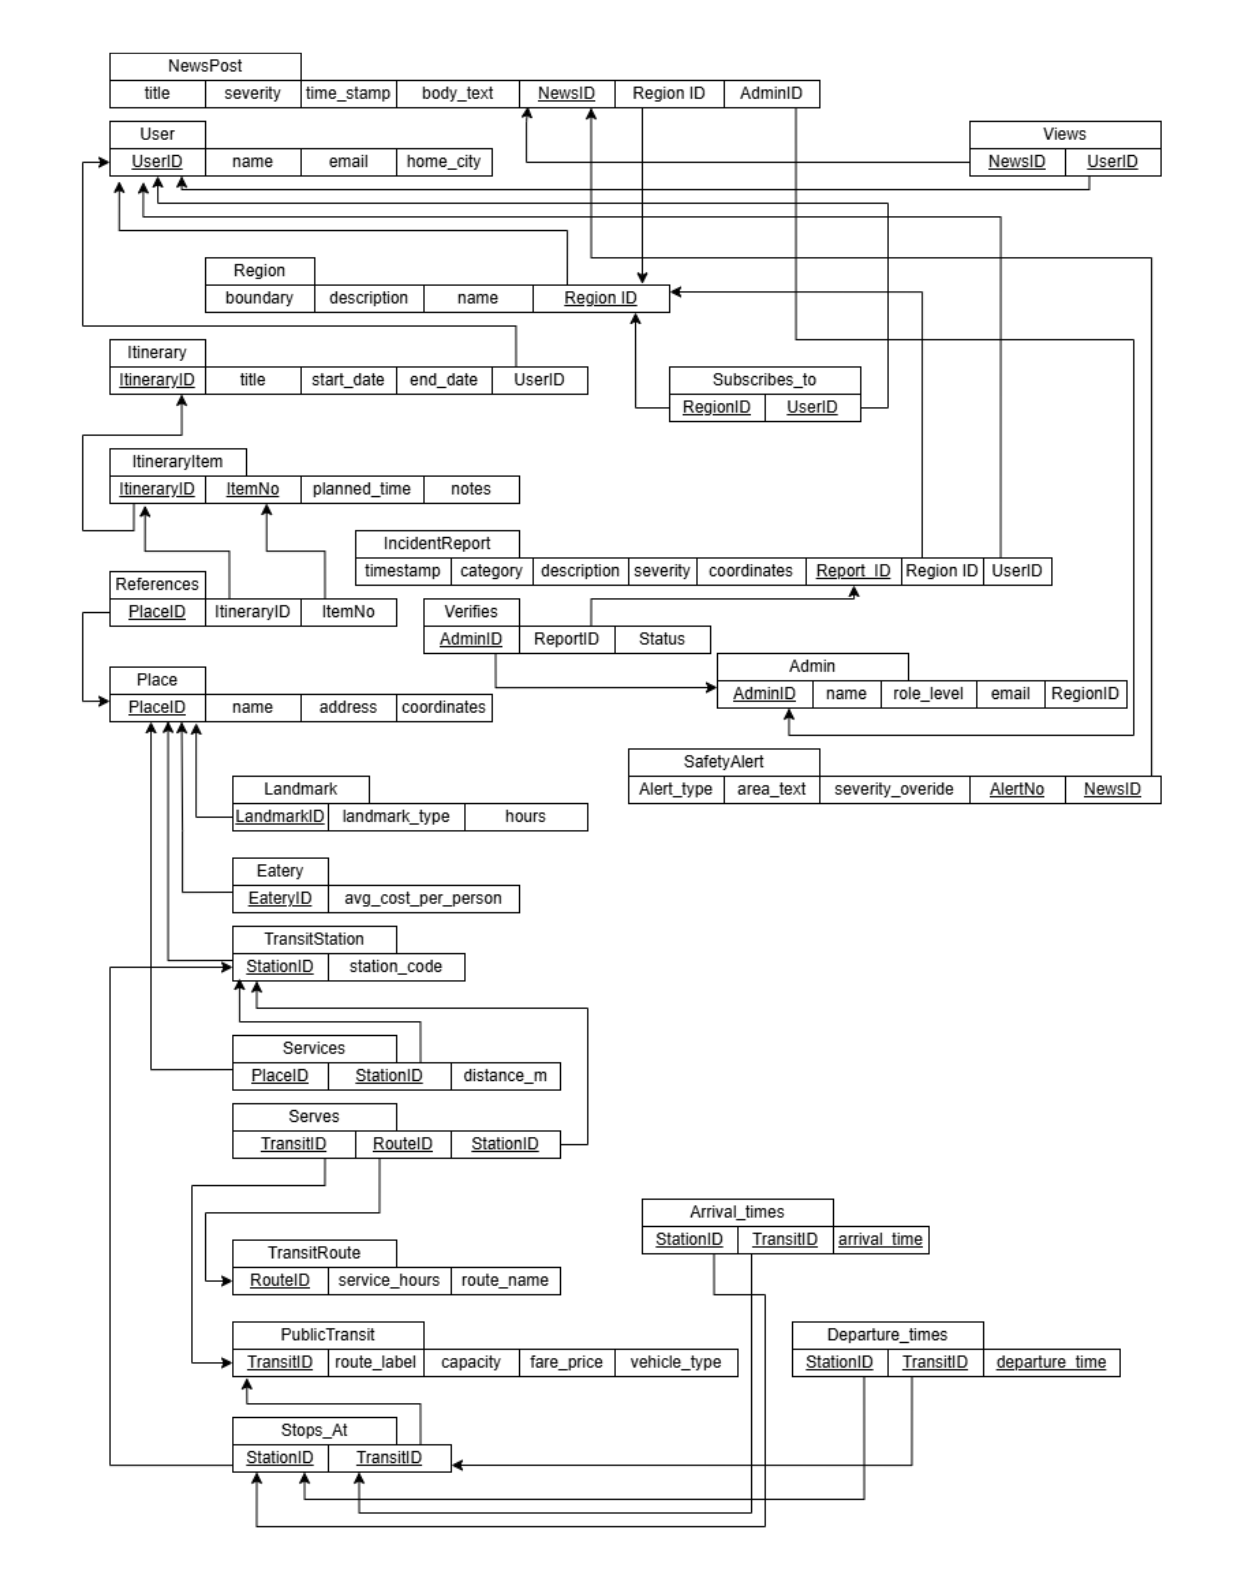
\includegraphics[width=\textwidth,height=0.9\textheight,keepaspectratio]{figures/relational-model.png}%
    }{%
        \fbox{\parbox{0.95\textwidth}{\centering\vspace{3cm}\textbf{Placeholder for Relational Model diagram}\\\vspace{0.3cm}This figure will show the relational schema diagram for Urban Scout, derived from the EER through the standard mapping algorithm. It will include all 25 tables with primary and foreign key relationships drawn out.\\\vspace{0.3cm}\texttt{figures/relational-model.png}\vspace{3cm}}}%
    }
    \caption{Relational schema diagram for Urban Scout.}
    \label{fig:rm}
\end{figure}

\begin{figure}[p]
    \centering
    \IfFileExists{figures/uml.png}{%
        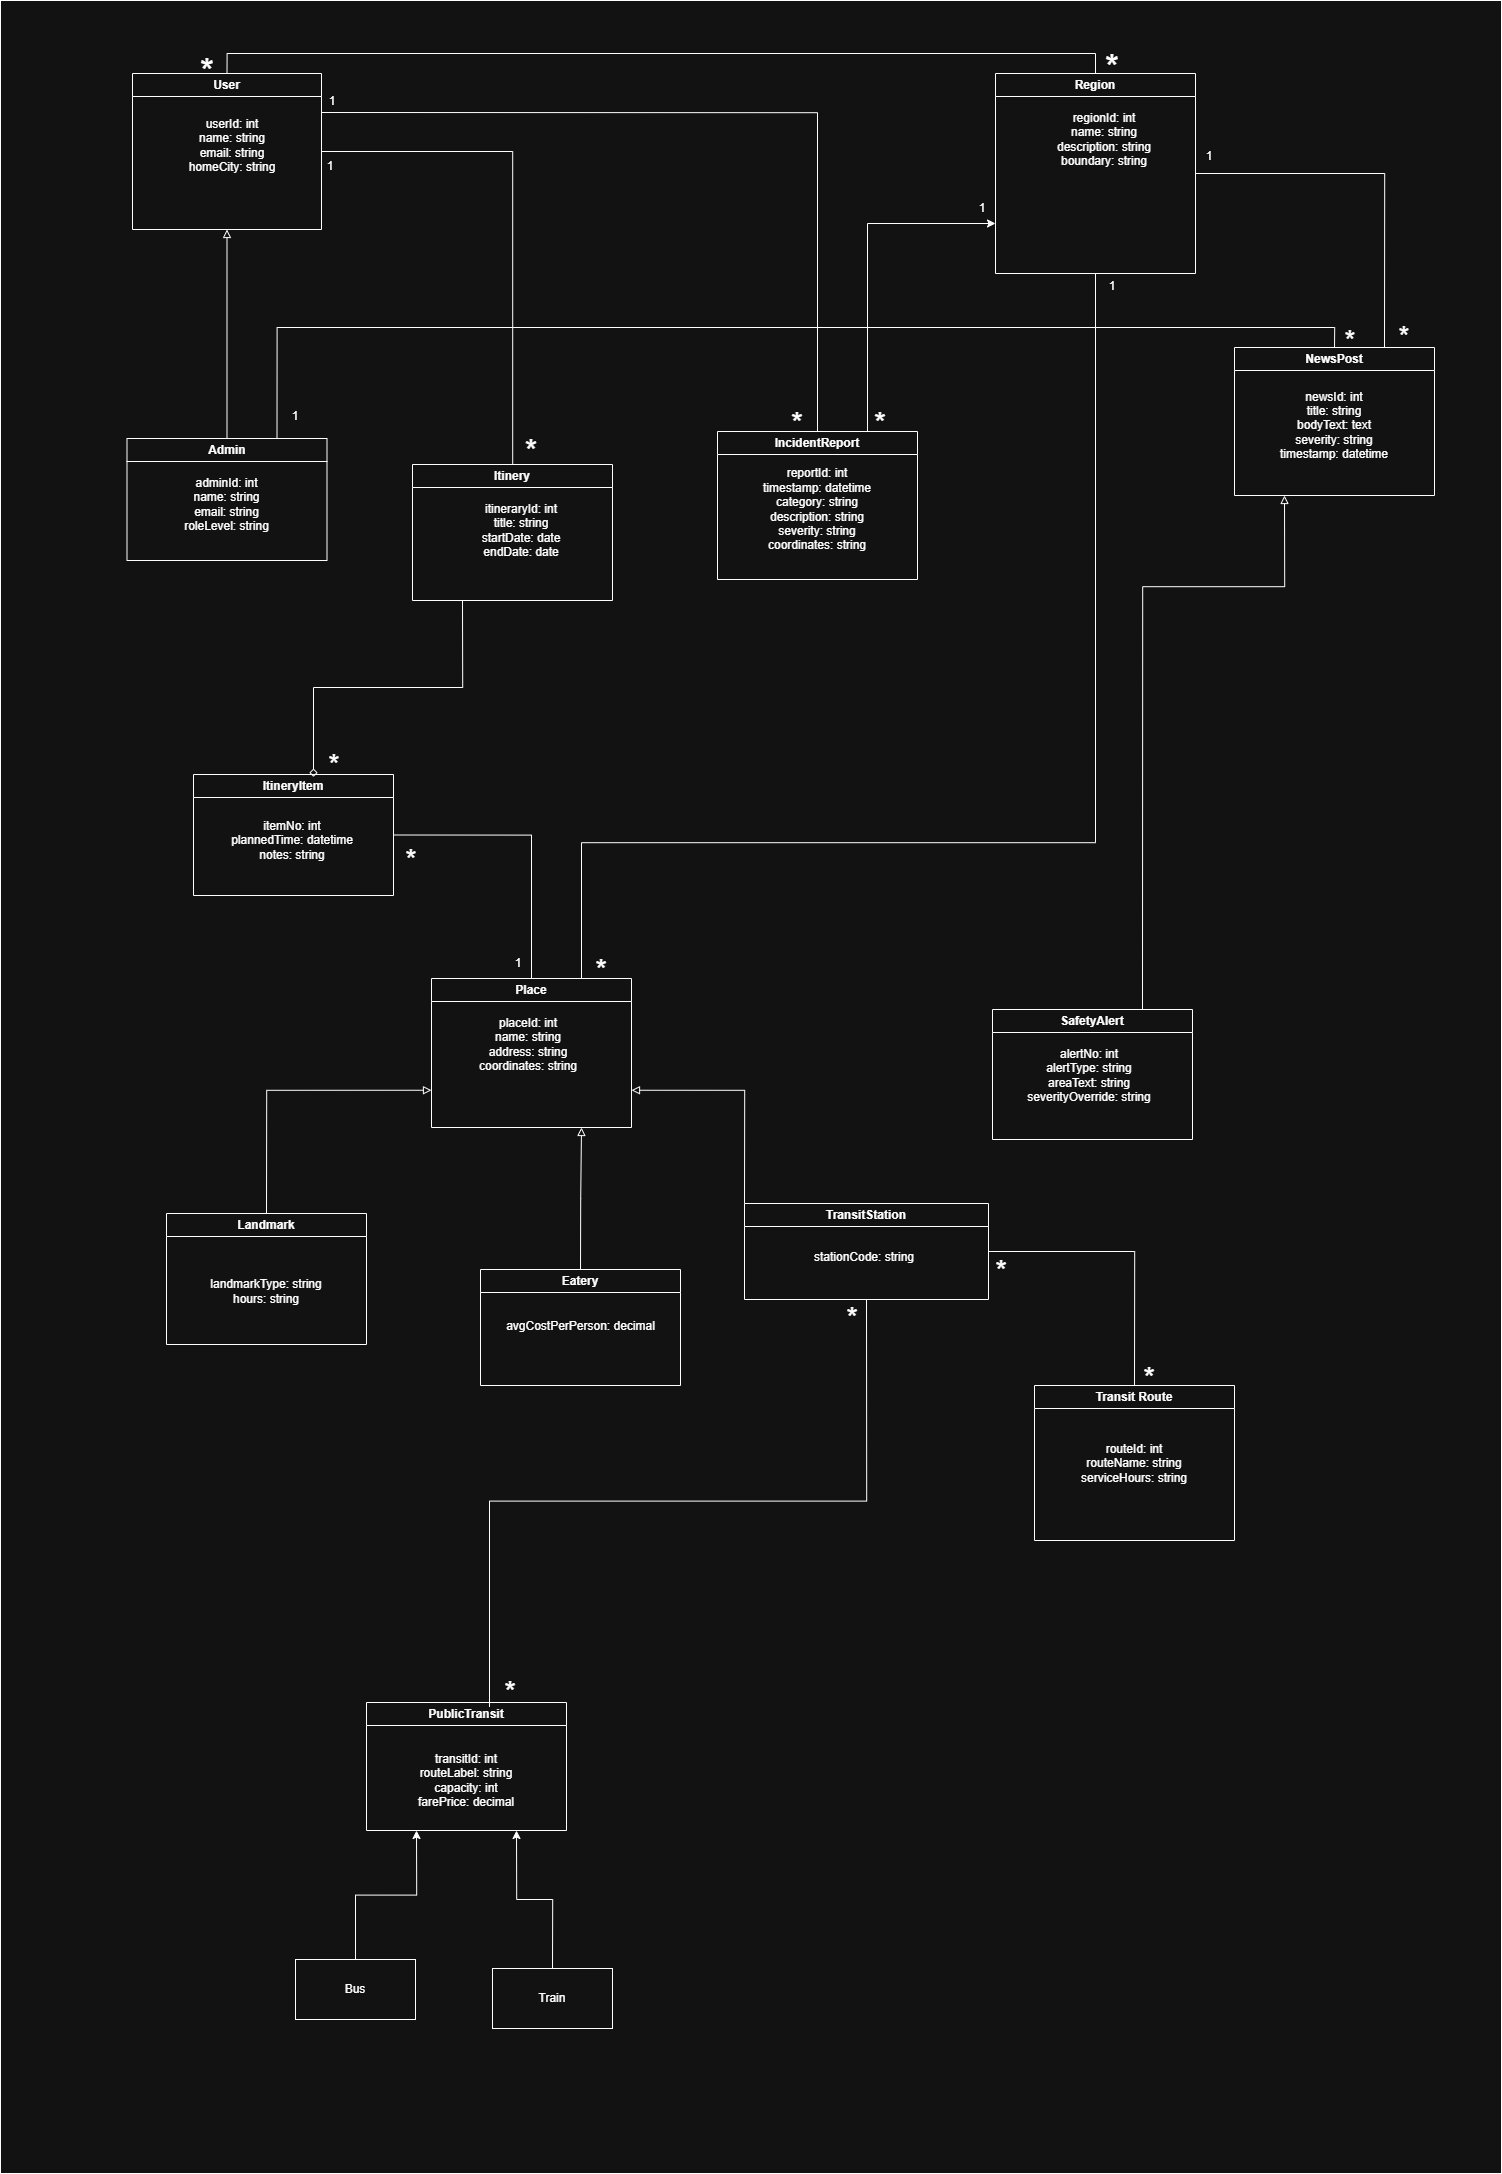
\includegraphics[width=\textwidth,height=0.9\textheight,keepaspectratio]{figures/uml.png}%
    }{%
        \fbox{\parbox{0.95\textwidth}{\centering\vspace{3cm}\textbf{Placeholder for UML class diagram}\\\vspace{0.3cm}This figure will show the UML class diagram for the Urban Scout relational model, displaying all entity classes with their attributes and inter-table relationships.\\\vspace{0.3cm}\texttt{figures/uml.png}\vspace{3cm}}}%
    }
    \caption{UML class diagram showing entity attributes and relationships.}
    \label{fig:uml}
\end{figure}

\subsection{Conversion from ER Diagram to Relational Schema}

The relational schema was created by following the standard ER-to-relational mapping approach.

\boldheading{Strong Entities}

Strong entities in the ER diagram were mapped directly into tables with primary keys. Examples include \texttt{User}, \texttt{Admin}, \texttt{Region}, \texttt{Place}, \texttt{TransitRoute}, \texttt{PublicTransit}, \texttt{NewsPost}, \texttt{IncidentReport}, and \texttt{Itinerary}. Each of these relations has its own primary key and stores attributes that belong directly to that entity.

\boldheading{Specialization}

One of the important design decisions in the project was the specialization of \texttt{Place} into \texttt{Landmark}, \texttt{Eatery}, and \texttt{TransitStation}. Instead of storing all place-specific attributes in a single large table, the implementation uses separate subtype tables. \texttt{Place} stores shared attributes such as name, address, coordinates, and region. \texttt{Landmark} stores landmark-specific data, \texttt{Eatery} stores eatery-specific data, and \texttt{TransitStation} stores station-specific data.

This design was chosen because it keeps the database normalized and avoids storing many null attributes in a single universal place table. It also reflects the conceptual distinction between different kinds of locations while preserving their shared identity.

\boldheading{Weak Entities}

Two important weak entities appear in the schema: \texttt{SafetyAlert} and \texttt{ItineraryItem}. \texttt{SafetyAlert} depends on \texttt{NewsPost}, so it was implemented with a composite key including the owning news post identifier and a local alert number. \texttt{ItineraryItem} depends on \texttt{Itinerary}, so it was implemented with a composite key including the itinerary identifier and an item number.

The use of weak entities was an important part of the project because it allowed the schema to represent dependent data in a structured and relationally correct way.

\boldheading{Many-to-Many Relationships}

Several many-to-many relationships in the ER diagram were converted into separate associative tables. These include user subscriptions to regions, itinerary items referencing places, routes serving stations through transit services, places being near transit stations, users viewing news posts, and administrators verifying incident reports.

These relationships were implemented through linking tables such as \texttt{Subscribes\_to}, \texttt{References}, \texttt{Serves}, \texttt{Services}, \texttt{Views}, and \texttt{Verifies}. This decision was necessary because many-to-many relationships cannot be represented directly in a normalized relational schema without introducing a separate relation.

\subsection{Significant Design Decisions}

Several implementation decisions were especially important during the conversion process.

\boldheading{Use of Separate Admin and User Tables}

The project keeps \texttt{User} and \texttt{Admin} as separate tables rather than placing both roles into one shared account table. This was done to keep the distinction between tourists and administrators explicit in both the schema and the application logic. Because the two user types have different roles and responsibilities, separating them simplified access control and role-based routing in the backend.

\boldheading{Modeling Transit with Multiple Related Tables}

Transit information was not stored in a single table. Instead, the design separates transit services (\texttt{PublicTransit}), route information (\texttt{TransitRoute}), stations (\texttt{TransitStation}), station-route-service relationships (\texttt{Serves}), stop relationships (\texttt{Stops\_At}), and arrival and departure schedules (\texttt{Arrival\_times}, \texttt{Departure\_times}).

This decision increased the complexity of the schema, but it allowed the project to model the transit system in a much more realistic way. It also supported one of the project's showcase queries: retrieving the full schedule and service information for a selected station.

\boldheading{Region-Centered Organization}

Another major implementation choice was to make \texttt{Region} a central organizing entity. Instead of treating the city as a single undifferentiated space, the schema uses regions to group places, news, subscriptions, reports, and administrative responsibilities. This makes filtering and personalization much easier in the application.

\subsection{DBMS Selection}

The project was implemented using \textbf{MySQL} as the DBMS.

MySQL was selected for several reasons:
\begin{itemize}
    \item it is a widely used relational database system
    \item it aligns well with the course focus on SQL and relational database design
    \item it supports foreign keys, joins, procedures, and indexing features needed for the project
    \item it integrates smoothly with the Node.js backend using the \texttt{mysql2} library
    \item it is accessible and practical for local development and demonstration
\end{itemize}

Because the project emphasizes database concepts, MySQL was an appropriate choice. It allowed the team to implement the schema directly in SQL and demonstrate clear understanding of relational modeling, rather than relying on an abstraction layer such as an ORM.

\subsection{Database Implementation}

The database implementation was organized through SQL scripts that define the schema, insert sample data, and create stored procedures.

The implementation includes:
\begin{itemize}
    \item a schema script to create all relations and constraints
    \item a seed script to populate the database with sample data
    \item a script for stored procedures
    \item a drop/reset script used during testing and redevelopment
\end{itemize}
\nopagebreak[4]

\noindent This structure made the project easier to maintain and reset during development. It also ensured that the same database could be recreated consistently for testing, demo preparation, and final submission.

\boldheading{Schema Definition (DDL)}

\begin{lstlisting}[language=MySQL,caption={Full database schema (DDL).},label={lst:ddl}]
-- Urban Scout - CPSC 471 Group 61 - Database Schema (MySQL 8.0)

CREATE DATABASE IF NOT EXISTS UrbanScout;
USE UrbanScout;

CREATE TABLE User (
    UserID      INT             PRIMARY KEY AUTO_INCREMENT,
    name        VARCHAR(100)    NOT NULL,
    email       VARCHAR(150)    NOT NULL UNIQUE,
    home_city   VARCHAR(100)
);

CREATE TABLE Region (
    RegionID    INT             PRIMARY KEY AUTO_INCREMENT,
    name        VARCHAR(100)    NOT NULL,
    description TEXT,
    boundary    VARCHAR(255)
);

CREATE TABLE Admin (
    AdminID     INT             PRIMARY KEY AUTO_INCREMENT,
    name        VARCHAR(100)    NOT NULL,
    email       VARCHAR(150)    NOT NULL UNIQUE,
    role_level  VARCHAR(50),
    RegionID    INT             NOT NULL,
    FOREIGN KEY (RegionID) REFERENCES Region(RegionID)
        ON DELETE RESTRICT ON UPDATE CASCADE
);

CREATE TABLE Place (
    PlaceID     INT             PRIMARY KEY AUTO_INCREMENT,
    name        VARCHAR(150)    NOT NULL,
    address     VARCHAR(255),
    coordinates VARCHAR(50),
    RegionID    INT             NOT NULL,
    FOREIGN KEY (RegionID) REFERENCES Region(RegionID)
        ON DELETE RESTRICT ON UPDATE CASCADE
);

CREATE TABLE Landmark (
    LandmarkID      INT         PRIMARY KEY,
    landmark_type   VARCHAR(50),
    hours           VARCHAR(100),
    FOREIGN KEY (LandmarkID) REFERENCES Place(PlaceID)
        ON DELETE CASCADE ON UPDATE CASCADE
);

CREATE TABLE Eatery (
    EateryID            INT             PRIMARY KEY,
    avg_cost_per_person DECIMAL(8,2),
    FOREIGN KEY (EateryID) REFERENCES Place(PlaceID)
        ON DELETE CASCADE ON UPDATE CASCADE
);

CREATE TABLE TransitStation (
    StationID       INT         PRIMARY KEY,
    station_code    VARCHAR(20),
    FOREIGN KEY (StationID) REFERENCES Place(PlaceID)
        ON DELETE CASCADE ON UPDATE CASCADE
);

CREATE TABLE TransitRoute (
    RouteID         INT             PRIMARY KEY AUTO_INCREMENT,
    route_name      VARCHAR(100)    NOT NULL,
    service_hours   VARCHAR(100)
);

CREATE TABLE PublicTransit (
    TransitID       INT             PRIMARY KEY AUTO_INCREMENT,
    route_label     VARCHAR(50),
    capacity        INT,
    fare_price      DECIMAL(6,2),
    vehicle_type    VARCHAR(20)
);

CREATE TABLE Bus (
    TransitID       INT         PRIMARY KEY,
    bus_number      VARCHAR(20),
    FOREIGN KEY (TransitID) REFERENCES PublicTransit(TransitID)
        ON DELETE CASCADE ON UPDATE CASCADE
);

CREATE TABLE Train (
    TransitID       INT         PRIMARY KEY,
    car_count       INT,
    FOREIGN KEY (TransitID) REFERENCES PublicTransit(TransitID)
        ON DELETE CASCADE ON UPDATE CASCADE
);

CREATE TABLE NewsPost (
    NewsID      INT             PRIMARY KEY AUTO_INCREMENT,
    title       VARCHAR(200)    NOT NULL,
    severity    VARCHAR(20),
    time_stamp  DATETIME        NOT NULL DEFAULT CURRENT_TIMESTAMP,
    body_text   TEXT,
    RegionID    INT             NOT NULL,
    AdminID     INT             NOT NULL,
    FOREIGN KEY (RegionID) REFERENCES Region(RegionID)
        ON DELETE RESTRICT ON UPDATE CASCADE,
    FOREIGN KEY (AdminID) REFERENCES Admin(AdminID)
        ON DELETE RESTRICT ON UPDATE CASCADE
);

CREATE TABLE SafetyAlert (
    NewsID              INT             NOT NULL,
    AlertNo             INT             NOT NULL,
    alert_type          VARCHAR(50),
    area_text           VARCHAR(255),
    severity_override   VARCHAR(20),
    PRIMARY KEY (NewsID, AlertNo),
    FOREIGN KEY (NewsID) REFERENCES NewsPost(NewsID)
        ON DELETE CASCADE ON UPDATE CASCADE
);

CREATE TABLE IncidentReport (
    Report_ID   INT             PRIMARY KEY AUTO_INCREMENT,
    timestamp   DATETIME        NOT NULL DEFAULT CURRENT_TIMESTAMP,
    category    VARCHAR(50),
    description TEXT,
    severity    VARCHAR(20),
    coordinates VARCHAR(50),
    UserID      INT             NOT NULL,
    RegionID    INT             NOT NULL,
    FOREIGN KEY (UserID) REFERENCES User(UserID)
        ON DELETE CASCADE ON UPDATE CASCADE,
    FOREIGN KEY (RegionID) REFERENCES Region(RegionID)
        ON DELETE RESTRICT ON UPDATE CASCADE
);

CREATE TABLE Itinerary (
    ItineraryID INT             PRIMARY KEY AUTO_INCREMENT,
    title       VARCHAR(150)    NOT NULL,
    start_date  DATE,
    end_date    DATE,
    UserID      INT             NOT NULL,
    FOREIGN KEY (UserID) REFERENCES User(UserID)
        ON DELETE CASCADE ON UPDATE CASCADE
);

CREATE TABLE ItineraryItem (
    ItineraryID INT         NOT NULL,
    ItemNo      INT         NOT NULL,
    planned_time DATETIME,
    notes       TEXT,
    PRIMARY KEY (ItineraryID, ItemNo),
    FOREIGN KEY (ItineraryID) REFERENCES Itinerary(ItineraryID)
        ON DELETE CASCADE ON UPDATE CASCADE
);

CREATE TABLE `References` (
    PlaceID     INT     NOT NULL,
    ItineraryID INT     NOT NULL,
    ItemNo      INT     NOT NULL,
    PRIMARY KEY (PlaceID, ItineraryID, ItemNo),
    FOREIGN KEY (PlaceID)       REFERENCES Place(PlaceID)
        ON DELETE CASCADE ON UPDATE CASCADE,
    FOREIGN KEY (ItineraryID, ItemNo) REFERENCES ItineraryItem(ItineraryID, ItemNo)
        ON DELETE CASCADE ON UPDATE CASCADE
);

CREATE TABLE Subscribes_to (
    UserID      INT     NOT NULL,
    RegionID    INT     NOT NULL,
    PRIMARY KEY (UserID, RegionID),
    FOREIGN KEY (UserID)    REFERENCES User(UserID)
        ON DELETE CASCADE ON UPDATE CASCADE,
    FOREIGN KEY (RegionID)  REFERENCES Region(RegionID)
        ON DELETE CASCADE ON UPDATE CASCADE
);

CREATE TABLE Views (
    UserID  INT     NOT NULL,
    NewsID  INT     NOT NULL,
    PRIMARY KEY (UserID, NewsID),
    FOREIGN KEY (UserID) REFERENCES User(UserID)
        ON DELETE CASCADE ON UPDATE CASCADE,
    FOREIGN KEY (NewsID) REFERENCES NewsPost(NewsID)
        ON DELETE CASCADE ON UPDATE CASCADE
);

CREATE TABLE Verifies (
    AdminID     INT             NOT NULL,
    ReportID    INT             NOT NULL,
    Status      VARCHAR(30)     NOT NULL DEFAULT 'pending',
    PRIMARY KEY (AdminID, ReportID),
    FOREIGN KEY (AdminID)   REFERENCES Admin(AdminID)
        ON DELETE CASCADE ON UPDATE CASCADE,
    FOREIGN KEY (ReportID)  REFERENCES IncidentReport(Report_ID)
        ON DELETE CASCADE ON UPDATE CASCADE
);

CREATE TABLE Services (
    PlaceID     INT             NOT NULL,
    StationID   INT             NOT NULL,
    distance_m  DECIMAL(8,1),
    PRIMARY KEY (PlaceID, StationID),
    FOREIGN KEY (PlaceID)   REFERENCES Place(PlaceID)
        ON DELETE CASCADE ON UPDATE CASCADE,
    FOREIGN KEY (StationID) REFERENCES TransitStation(StationID)
        ON DELETE CASCADE ON UPDATE CASCADE
);

CREATE TABLE Serves (
    RouteID     INT     NOT NULL,
    StationID   INT     NOT NULL,
    TransitID   INT     NOT NULL,
    PRIMARY KEY (RouteID, StationID, TransitID),
    FOREIGN KEY (RouteID)   REFERENCES TransitRoute(RouteID)
        ON DELETE CASCADE ON UPDATE CASCADE,
    FOREIGN KEY (StationID) REFERENCES TransitStation(StationID)
        ON DELETE CASCADE ON UPDATE CASCADE,
    FOREIGN KEY (TransitID) REFERENCES PublicTransit(TransitID)
        ON DELETE CASCADE ON UPDATE CASCADE
);

CREATE TABLE Stops_At (
    StationID   INT     NOT NULL,
    TransitID   INT     NOT NULL,
    PRIMARY KEY (StationID, TransitID),
    FOREIGN KEY (StationID) REFERENCES TransitStation(StationID)
        ON DELETE CASCADE ON UPDATE CASCADE,
    FOREIGN KEY (TransitID) REFERENCES PublicTransit(TransitID)
        ON DELETE CASCADE ON UPDATE CASCADE
);

CREATE TABLE Arrival_times (
    TransitID       INT     NOT NULL,
    StationID       INT     NOT NULL,
    arrival_time    TIME    NOT NULL,
    PRIMARY KEY (TransitID, StationID, arrival_time),
    FOREIGN KEY (TransitID) REFERENCES PublicTransit(TransitID)
        ON DELETE CASCADE ON UPDATE CASCADE,
    FOREIGN KEY (StationID) REFERENCES TransitStation(StationID)
        ON DELETE CASCADE ON UPDATE CASCADE
);

CREATE TABLE Departure_times (
    TransitID       INT     NOT NULL,
    StationID       INT     NOT NULL,
    departure_time  TIME    NOT NULL,
    PRIMARY KEY (TransitID, StationID, departure_time),
    FOREIGN KEY (TransitID) REFERENCES PublicTransit(TransitID)
        ON DELETE CASCADE ON UPDATE CASCADE,
    FOREIGN KEY (StationID) REFERENCES TransitStation(StationID)
        ON DELETE CASCADE ON UPDATE CASCADE
);
\end{lstlisting}

\subsection{Transactions and SQL Statements}

The application exposes 36 REST endpoints across 8 route modules. Each endpoint maps to one or more SQL statements that are executed using \texttt{mysql2} prepared statements. The complete list grouped by feature area follows below.

\subsubsection{Authentication}

\textbf{POST /api/auth/register} \textit{(Auth: none.)}
Creates a new user account and saves the user to the session.
\begin{lstlisting}[language=MySQL]
INSERT INTO User (name, email, home_city) VALUES (?, ?, ?);
\end{lstlisting}

\textbf{POST /api/auth/login} \textit{(Auth: none.)}
Looks up a user by email and establishes a session.
\begin{lstlisting}[language=MySQL]
SELECT * FROM User WHERE email = ?;
\end{lstlisting}

\textbf{POST /api/auth/admin-login} \textit{(Auth: none.)}
Looks up an admin by email and establishes an admin session.
\begin{lstlisting}[language=MySQL]
SELECT * FROM Admin WHERE email = ?;
\end{lstlisting}

\textbf{POST /api/auth/logout} \textit{(Auth: none.)}
Destroys the current session.
\textit{No SQL is executed. The handler only clears the session.}

\textbf{GET /api/auth/me} \textit{(Auth: none.)}
Returns the currently logged-in user or admin, or null if no session is active.
\textit{No SQL is executed. The handler only inspects the session.}

\subsubsection{Regions}

\textbf{GET /api/regions} \textit{(Auth: none.)}
Retrieves all regions for the home page.
\begin{lstlisting}[language=MySQL]
SELECT * FROM Region;
\end{lstlisting}

\textbf{GET /api/regions/:id} \textit{(Auth: none.)}
Retrieves a single region together with its place count and news post count.
\begin{lstlisting}[language=MySQL]
SELECT * FROM Region WHERE RegionID = ?;
SELECT COUNT(*) as count FROM Place WHERE RegionID = ?;
SELECT COUNT(*) as count FROM NewsPost WHERE RegionID = ?;
\end{lstlisting}

\subsubsection{Places}

\textbf{GET /api/places} \textit{(Auth: none.)}
Retrieves all places, optionally filtered by region and place type. The handler picks one of four query branches based on the type parameter.
\begin{lstlisting}[language=MySQL]
-- when type=landmark
SELECT p.*, l.landmark_type, l.hours
FROM Place p JOIN Landmark l ON p.PlaceID = l.LandmarkID
WHERE 1=1 ORDER BY p.name;

-- when type=eatery
SELECT p.*, e.avg_cost_per_person
FROM Place p JOIN Eatery e ON p.PlaceID = e.EateryID
WHERE 1=1 ORDER BY p.name;

-- when type=transit
SELECT p.*, ts.station_code
FROM Place p JOIN TransitStation ts ON p.PlaceID = ts.StationID
WHERE 1=1 ORDER BY p.name;

-- when no type filter
SELECT p.*,
  CASE
    WHEN l.LandmarkID IS NOT NULL THEN 'landmark'
    WHEN e.EateryID IS NOT NULL THEN 'eatery'
    WHEN ts.StationID IS NOT NULL THEN 'transit'
    ELSE 'other'
  END AS placeType,
  l.landmark_type, l.hours,
  e.avg_cost_per_person,
  ts.station_code
FROM Place p
LEFT JOIN Landmark l ON p.PlaceID = l.LandmarkID
LEFT JOIN Eatery e ON p.PlaceID = e.EateryID
LEFT JOIN TransitStation ts ON p.PlaceID = ts.StationID
WHERE 1=1 ORDER BY p.name;

-- regionId filter appended:
-- AND p.RegionID = ?
\end{lstlisting}

\textbf{GET /api/places/:id} \textit{(Auth: none.)}
Retrieves a single place along with its specialization details and any nearby transit stations.
\begin{lstlisting}[language=MySQL]
SELECT p.*,
  l.landmark_type, l.hours,
  e.avg_cost_per_person,
  ts.station_code,
  CASE
    WHEN l.LandmarkID IS NOT NULL THEN 'landmark'
    WHEN e.EateryID IS NOT NULL THEN 'eatery'
    WHEN ts.StationID IS NOT NULL THEN 'transit'
    ELSE 'other'
  END AS placeType
FROM Place p
LEFT JOIN Landmark l ON p.PlaceID = l.LandmarkID
LEFT JOIN Eatery e ON p.PlaceID = e.EateryID
LEFT JOIN TransitStation ts ON p.PlaceID = ts.StationID
WHERE p.PlaceID = ?;

SELECT s.distance_m, p.name AS station_name, ts.station_code, p.PlaceID AS StationPlaceID
FROM Services s
JOIN Place p ON s.StationID = p.PlaceID
JOIN TransitStation ts ON s.StationID = ts.StationID
WHERE s.PlaceID = ?
ORDER BY s.distance_m ASC;
\end{lstlisting}

\textbf{POST /api/places} \textit{(Auth: admin.)}
Creates a new place along with its specialization row inside a single transaction so the parent and subtype rows stay in sync.
\begin{lstlisting}[language=MySQL]
START TRANSACTION;

INSERT INTO Place (name, address, coordinates, RegionID)
VALUES (?, ?, ?, ?);

-- one of the following depending on type
INSERT INTO Landmark (LandmarkID, landmark_type, hours) VALUES (?, ?, ?);
INSERT INTO Eatery (EateryID, avg_cost_per_person) VALUES (?, ?);
INSERT INTO TransitStation (StationID, station_code) VALUES (?, ?);

COMMIT;
\end{lstlisting}

\subsubsection{Transit}

\textbf{GET /api/transit/routes} \textit{(Auth: none.)}
Retrieves all transit routes.
\begin{lstlisting}[language=MySQL]
SELECT * FROM TransitRoute;
\end{lstlisting}

\textbf{POST /api/transit/routes} \textit{(Auth: admin.)}
Adds a new transit route.
\begin{lstlisting}[language=MySQL]
INSERT INTO TransitRoute (route_name, service_hours) VALUES (?, ?);
\end{lstlisting}

\textbf{DELETE /api/transit/routes/:id} \textit{(Auth: admin.)}
Deletes a transit route. The deletion cascades to the \texttt{Serves} junction table.
\begin{lstlisting}[language=MySQL]
DELETE FROM TransitRoute WHERE RouteID = ?;
\end{lstlisting}

\textbf{POST /api/transit/routes/:id/stations} \textit{(Auth: admin.)}
Links a station and a transit vehicle to a route as a stop.
\begin{lstlisting}[language=MySQL]
INSERT INTO Serves (RouteID, StationID, TransitID) VALUES (?, ?, ?);
\end{lstlisting}

\textbf{DELETE /api/transit/routes/:id/stations} \textit{(Auth: admin.)}
Removes a stop from a route.
\begin{lstlisting}[language=MySQL]
DELETE FROM Serves WHERE RouteID = ? AND StationID = ? AND TransitID = ?;
\end{lstlisting}

\textbf{GET /api/transit/routes/:id/stations} \textit{(Auth: none.)}
Lists the stops on a single route, joining station and vehicle information for display.
\begin{lstlisting}[language=MySQL]
SELECT sv.StationID, sv.TransitID,
       p.name AS station_name, ts.station_code,
       pt.route_label, pt.vehicle_type
FROM Serves sv
JOIN TransitStation ts ON sv.StationID = ts.StationID
JOIN Place p ON ts.StationID = p.PlaceID
JOIN PublicTransit pt ON sv.TransitID = pt.TransitID
WHERE sv.RouteID = ?
ORDER BY p.name;
\end{lstlisting}

\textbf{GET /api/transit/vehicles} \textit{(Auth: none.)}
Lists transit vehicles, with an optional vehicle type filter.
\begin{lstlisting}[language=MySQL]
SELECT * FROM PublicTransit;
-- with type filter:
SELECT * FROM PublicTransit WHERE vehicle_type = ?;
\end{lstlisting}

\textbf{GET /api/transit/stations/:id/schedule} \textit{(Auth: none.)}
Returns four result sets that together make up a station's schedule view: station info, arrivals, departures, and the routes that serve the station.
\begin{lstlisting}[language=MySQL]
SELECT p.name, p.address, p.coordinates, ts.station_code
FROM Place p JOIN TransitStation ts ON p.PlaceID = ts.StationID
WHERE ts.StationID = ?;

SELECT at.arrival_time, pt.route_label, pt.vehicle_type, pt.TransitID
FROM Arrival_times at JOIN PublicTransit pt ON at.TransitID = pt.TransitID
WHERE at.StationID = ?
ORDER BY at.arrival_time;

SELECT dt.departure_time, pt.route_label, pt.vehicle_type, pt.TransitID
FROM Departure_times dt JOIN PublicTransit pt ON dt.TransitID = pt.TransitID
WHERE dt.StationID = ?
ORDER BY dt.departure_time;

SELECT DISTINCT tr.RouteID, tr.route_name, tr.service_hours
FROM Serves sv JOIN TransitRoute tr ON sv.RouteID = tr.RouteID
WHERE sv.StationID = ?;
\end{lstlisting}

\textbf{GET /api/transit/stations/:id/nearby} \textit{(Auth: none.)}
Finds places within walking distance of a station by calling the \texttt{sp\_nearby\_places} stored procedure.
\begin{lstlisting}[language=MySQL]
CALL sp_nearby_places(?, ?);
\end{lstlisting}

\subsubsection{News}

\textbf{GET /api/news} \textit{(Auth: none for public browse, but the session is consulted to filter by subscriptions when a user is logged in and no \texttt{regionId} is supplied.)}
Retrieves news posts together with embedded safety alerts. The handler picks one of three branches: a specific region, the logged-in user's subscribed regions, or all news.
\begin{lstlisting}[language=MySQL]
-- anonymous, all news
SELECT np.*, r.name AS region_name, a.name AS admin_name,
  sa.AlertNo, sa.alert_type, sa.area_text, sa.severity_override
FROM NewsPost np
JOIN Region r ON np.RegionID = r.RegionID
JOIN Admin a ON np.AdminID = a.AdminID
LEFT JOIN SafetyAlert sa ON np.NewsID = sa.NewsID
ORDER BY np.time_stamp DESC;

-- with regionId
... WHERE np.RegionID = ? ORDER BY np.time_stamp DESC;

-- logged-in user, no regionId, default to subscribed regions
... WHERE np.RegionID IN (
  SELECT RegionID FROM Subscribes_to WHERE UserID = ?
) ORDER BY np.time_stamp DESC;
\end{lstlisting}

\textbf{GET /api/news/:id} \textit{(Auth: none.)}
Retrieves a single news post and its safety alerts.
\begin{lstlisting}[language=MySQL]
SELECT np.*, r.name AS region_name, a.name AS admin_name
FROM NewsPost np
JOIN Region r ON np.RegionID = r.RegionID
JOIN Admin a ON np.AdminID = a.AdminID
WHERE np.NewsID = ?;

SELECT * FROM SafetyAlert WHERE NewsID = ?;
\end{lstlisting}

\textbf{POST /api/news} \textit{(Auth: admin.)}
Creates a news post and optionally attaches one safety alert.
\begin{lstlisting}[language=MySQL]
INSERT INTO NewsPost (title, severity, body_text, RegionID, AdminID) VALUES (?, ?, ?, ?, ?);
INSERT INTO SafetyAlert (NewsID, AlertNo, alert_type, area_text, severity_override) VALUES (?, 1, ?, ?, ?);
\end{lstlisting}

\textbf{POST /api/news/:id/view} \textit{(Auth: user.)}
Records that a user viewed a news post. Uses \texttt{INSERT IGNORE} so repeated views do not produce duplicate rows.
\begin{lstlisting}[language=MySQL]
INSERT IGNORE INTO Views (UserID, NewsID) VALUES (?, ?);
\end{lstlisting}

\subsubsection{Incidents}

\textbf{GET /api/incidents/mine} \textit{(Auth: user.)}
Lists the logged-in user's reports together with verification status from the \texttt{Verifies} junction table.
\begin{lstlisting}[language=MySQL]
SELECT ir.*, r.name AS region_name,
  v.Status AS verification_status, a.name AS verifier_name
FROM IncidentReport ir
JOIN Region r ON ir.RegionID = r.RegionID
LEFT JOIN Verifies v ON ir.Report_ID = v.ReportID
LEFT JOIN Admin a ON v.AdminID = a.AdminID
WHERE ir.UserID = ?
ORDER BY ir.timestamp DESC;
\end{lstlisting}

\textbf{GET /api/incidents} \textit{(Auth: none, but admins typically pass a \texttt{regionId} filter.)}
Lists reports, optionally filtered by region.
\begin{lstlisting}[language=MySQL]
SELECT ir.*, u.name AS reporter_name,
  v.AdminID AS verifier_id, v.Status AS verification_status,
  a.name AS verifier_name
FROM IncidentReport ir
JOIN User u ON ir.UserID = u.UserID
LEFT JOIN Verifies v ON ir.Report_ID = v.ReportID
LEFT JOIN Admin a ON v.AdminID = a.AdminID
ORDER BY ir.timestamp DESC;

-- with regionId filter:
... WHERE ir.RegionID = ? ORDER BY ir.timestamp DESC;
\end{lstlisting}

\textbf{POST /api/incidents} \textit{(Auth: user.)}
Submits a new incident report on behalf of the logged-in user.
\begin{lstlisting}[language=MySQL]
INSERT INTO IncidentReport (category, description, severity, coordinates, UserID, RegionID) VALUES (?, ?, ?, ?, ?, ?);
\end{lstlisting}

\textbf{PUT /api/incidents/:reportId/verify} \textit{(Auth: admin.)}
Verifies or rejects a report. \texttt{REPLACE INTO} handles the upsert so an admin can change a previous decision without manually deleting the old row.
\begin{lstlisting}[language=MySQL]
REPLACE INTO Verifies (AdminID, ReportID, Status) VALUES (?, ?, ?);
\end{lstlisting}

\subsubsection{Itineraries}

\textbf{GET /api/itineraries} \textit{(Auth: user.)}
Lists the user's itineraries, ordered by start date.
\begin{lstlisting}[language=MySQL]
SELECT * FROM Itinerary WHERE UserID = ? ORDER BY start_date DESC;
\end{lstlisting}

\textbf{GET /api/itineraries/:id} \textit{(Auth: user.)}
Retrieves one itinerary along with its items and any referenced places.
\begin{lstlisting}[language=MySQL]
SELECT * FROM Itinerary WHERE ItineraryID = ? AND UserID = ?;

SELECT ii.ItemNo, ii.planned_time, ii.notes,
  p.PlaceID, p.name AS place_name, p.address, p.coordinates
FROM ItineraryItem ii
LEFT JOIN `References` r ON ii.ItineraryID = r.ItineraryID AND ii.ItemNo = r.ItemNo
LEFT JOIN Place p ON r.PlaceID = p.PlaceID
WHERE ii.ItineraryID = ?
ORDER BY ii.planned_time;
\end{lstlisting}

\textbf{POST /api/itineraries} \textit{(Auth: user.)}
Creates a new itinerary owned by the logged-in user.
\begin{lstlisting}[language=MySQL]
INSERT INTO Itinerary (title, start_date, end_date, UserID) VALUES (?, ?, ?, ?);
\end{lstlisting}

\textbf{DELETE /api/itineraries/:id} \textit{(Auth: user.)}
Deletes an itinerary. The cascade rules clean up the itinerary's items and place references.
\begin{lstlisting}[language=MySQL]
DELETE FROM Itinerary WHERE ItineraryID = ? AND UserID = ?;
\end{lstlisting}

\textbf{POST /api/itineraries/:id/items} \textit{(Auth: user.)}
Adds an item to an itinerary, optionally linking it to a place. The handler first checks ownership, computes the next item number, inserts the item, and then writes the place reference if one was supplied.
\begin{lstlisting}[language=MySQL]
SELECT ItineraryID FROM Itinerary WHERE ItineraryID = ? AND UserID = ?;
SELECT COALESCE(MAX(ItemNo), 0) + 1 AS nextNo FROM ItineraryItem WHERE ItineraryID = ?;
INSERT INTO ItineraryItem (ItineraryID, ItemNo, planned_time, notes) VALUES (?, ?, ?, ?);
INSERT INTO `References` (PlaceID, ItineraryID, ItemNo) VALUES (?, ?, ?);
\end{lstlisting}

\textbf{PUT /api/itineraries/:id/items/:itemNo} \textit{(Auth: user.)}
Updates the planned time or notes for an existing item.
\begin{lstlisting}[language=MySQL]
UPDATE ItineraryItem SET planned_time = ?, notes = ? WHERE ItineraryID = ? AND ItemNo = ?;
\end{lstlisting}

\textbf{DELETE /api/itineraries/:id/items/:itemNo} \textit{(Auth: user.)}
Removes an item. The cascade rules also remove any matching rows in the \texttt{References} table.
\begin{lstlisting}[language=MySQL]
DELETE FROM ItineraryItem WHERE ItineraryID = ? AND ItemNo = ?;
\end{lstlisting}

\subsubsection{Subscriptions}

\textbf{GET /api/subscriptions} \textit{(Auth: user.)}
Lists the regions the user is subscribed to.
\begin{lstlisting}[language=MySQL]
SELECT r.*
FROM Subscribes_to st
JOIN Region r ON st.RegionID = r.RegionID
WHERE st.UserID = ?;
\end{lstlisting}

\textbf{POST /api/subscriptions} \textit{(Auth: user.)}
Subscribes the user to a region. \texttt{INSERT IGNORE} makes a duplicate request a no-op.
\begin{lstlisting}[language=MySQL]
INSERT IGNORE INTO Subscribes_to (UserID, RegionID) VALUES (?, ?);
\end{lstlisting}

\textbf{DELETE /api/subscriptions/:regionId} \textit{(Auth: user.)}
Unsubscribes the user from a region.
\begin{lstlisting}[language=MySQL]
DELETE FROM Subscribes_to WHERE UserID = ? AND RegionID = ?;
\end{lstlisting}

\begin{table}[H]
    \centering
    \caption{All API endpoints exposed by the backend.}
    \label{tab:endpoints}
    \begin{tabularx}{\textwidth}{l X l}
        \toprule
        \textbf{Method} & \textbf{Path} & \textbf{Auth} \\
        \midrule
        POST & /api/auth/register & none \\
        POST & /api/auth/login & none \\
        POST & /api/auth/admin-login & none \\
        POST & /api/auth/logout & none \\
        GET & /api/auth/me & none \\
        GET & /api/regions & none \\
        GET & /api/regions/:id & none \\
        GET & /api/places & none \\
        GET & /api/places/:id & none \\
        POST & /api/places & admin \\
        GET & /api/transit/routes & none \\
        POST & /api/transit/routes & admin \\
        DELETE & /api/transit/routes/:id & admin \\
        POST & /api/transit/routes/:id/stations & admin \\
        DELETE & /api/transit/routes/:id/stations & admin \\
        GET & /api/transit/routes/:id/stations & none \\
        GET & /api/transit/vehicles & none \\
        GET & /api/transit/stations/:id/schedule & none \\
        GET & /api/transit/stations/:id/nearby & none \\
        GET & /api/news & none \\
        GET & /api/news/:id & none \\
        POST & /api/news & admin \\
        POST & /api/news/:id/view & user \\
        GET & /api/incidents/mine & user \\
        GET & /api/incidents & none \\
        POST & /api/incidents & user \\
        PUT & /api/incidents/:reportId/verify & admin \\
        GET & /api/itineraries & user \\
        GET & /api/itineraries/:id & user \\
        POST & /api/itineraries & user \\
        DELETE & /api/itineraries/:id & user \\
        POST & /api/itineraries/:id/items & user \\
        PUT & /api/itineraries/:id/items/:itemNo & user \\
        DELETE & /api/itineraries/:id/items/:itemNo & user \\
        GET & /api/subscriptions & user \\
        POST & /api/subscriptions & user \\
        DELETE & /api/subscriptions/:regionId & user \\
        \bottomrule
    \end{tabularx}
\end{table}

\subsection{Stored Procedures and Special Queries}

Nine stored procedures are defined in the database to support common workflows. They cover registration, place lookup with optional type filtering, atomic itinerary creation from a JSON payload, admin verification of incident reports, walking-distance search for nearby places, multi-result-set transit schedules, personalized news feeds, popularity ranking, and region summaries. The API currently invokes \texttt{sp\_nearby\_places} for the transit station nearby places lookup. The remaining procedures are present in the database layer to support extended functionality and to demonstrate the procedural SQL capabilities of MySQL.

\subsubsection{sp\_register\_user}

This procedure inserts a new user into the \texttt{User} table inside a transaction and then returns the freshly created row using \texttt{LAST\_INSERT\_ID()}. It lets the API caller hand the new user details straight to the session without a follow-up query.

\begin{itemize}
    \item \textbf{Signature:} \texttt{IN p\_name VARCHAR(100), IN p\_email VARCHAR(150), IN p\_home\_city VARCHAR(100)}
    \item \textbf{Transactions used:} \texttt{START TRANSACTION} / \texttt{COMMIT}
    \item \textbf{Error handling:} none explicit
    \item \textbf{Result sets:} 1 (the new \texttt{User} row)
    \item \textbf{Called from API:} no, defined for completeness
\end{itemize}

\subsubsection{sp\_get\_places\_by\_region}

This procedure returns all places in a region, optionally filtered to landmarks, eateries, or transit stations. When no type is given, the result includes a \texttt{CASE}-derived \texttt{placeType} column so the caller knows what each row represents.

\begin{itemize}
    \item \textbf{Signature:} \texttt{IN p\_region\_id INT, IN p\_place\_type VARCHAR(20)}
    \item \textbf{Transactions used:} none
    \item \textbf{Error handling:} none
    \item \textbf{Result sets:} 1
    \item \textbf{Called from API:} no
\end{itemize}

\subsubsection{sp\_create\_itinerary\_with\_items}

This procedure creates an itinerary header plus all of its items in a single atomic operation. It accepts a JSON array of items, each with a \texttt{planned\_time}, \texttt{notes}, and optional \texttt{placeId}. If a \texttt{placeId} is present the procedure also writes a row in \texttt{References} to link the item to a place.

\begin{itemize}
    \item \textbf{Signature:} \texttt{IN p\_user\_id INT, IN p\_title VARCHAR(150), IN p\_start\_date DATE, IN p\_end\_date DATE, IN p\_items JSON}
    \item \textbf{Transactions used:} \texttt{START TRANSACTION} / \texttt{COMMIT} / \texttt{ROLLBACK}
    \item \textbf{Error handling:} \texttt{DECLARE EXIT HANDLER FOR SQLEXCEPTION}
    \item \textbf{Result sets:} 1 (the new \texttt{Itinerary} row)
    \item \textbf{Called from API:} no
\end{itemize}

\subsubsection{sp\_verify\_incident}

This procedure lets an admin confirm or reject an incident report. If the status is confirmed and the admin opts in, the procedure auto-publishes a \texttt{NewsPost} using the incident's category, description, severity, and region so subscribers see the alert without an extra API call.

\begin{itemize}
    \item \textbf{Signature:} \texttt{IN p\_admin\_id INT, IN p\_report\_id INT, IN p\_status VARCHAR(30), IN p\_create\_news BOOLEAN}
    \item \textbf{Transactions used:} \texttt{START TRANSACTION} / \texttt{COMMIT} / \texttt{ROLLBACK}
    \item \textbf{Error handling:} \texttt{DECLARE EXIT HANDLER FOR SQLEXCEPTION}
    \item \textbf{Result sets:} 1 (status message)
    \item \textbf{Called from API:} no
\end{itemize}

\subsubsection{sp\_nearby\_places}

This procedure returns every place within a walking-distance threshold of a given transit station. It uses the precomputed distances in the \texttt{Services} table so the lookup is a quick filtered \texttt{JOIN} rather than a runtime distance calculation. Each row includes the place type so the client knows whether it is a landmark, eatery, or another station.

\begin{itemize}
    \item \textbf{Signature:} \texttt{IN p\_station\_id INT, IN p\_max\_distance DECIMAL(8,1)}
    \item \textbf{Transactions used:} none needed (read-only)
    \item \textbf{Error handling:} none
    \item \textbf{Result sets:} 1
    \item \textbf{Called from API:} yes, at \texttt{server/routes/transit.js GET /api/transit/stations/:id/nearby}
\end{itemize}

\subsubsection{sp\_get\_transit\_schedule}

This procedure returns the full schedule view for one station as four sequential result sets. It demonstrates how a stored procedure can package multiple related queries that the application would otherwise have to issue separately.

\begin{itemize}
    \item \textbf{Signature:} \texttt{IN p\_station\_id INT}
    \item \textbf{Transactions used:} none
    \item \textbf{Error handling:} none
    \item \textbf{Result sets:} 4 (station info, serving routes, arrivals, departures)
    \item \textbf{Called from API:} no
\end{itemize}

\subsubsection{sp\_get\_user\_feed}

This procedure builds a personalized news feed for a user by pulling every \texttt{NewsPost} from the regions they subscribed to. Safety alerts attached to each post come along through a \texttt{LEFT JOIN} so the client can render them inline. Posts are returned in reverse chronological order.

\begin{itemize}
    \item \textbf{Signature:} \texttt{IN p\_user\_id INT}
    \item \textbf{Transactions used:} none
    \item \textbf{Error handling:} none
    \item \textbf{Result sets:} 1
    \item \textbf{Called from API:} no
\end{itemize}

\subsubsection{sp\_get\_popular\_places}

This procedure ranks places by how many times they appear in user itineraries through the \texttt{References} table and returns the top N. It is useful for trending or recommended lists across the app.

\begin{itemize}
    \item \textbf{Signature:} \texttt{IN p\_limit INT}
    \item \textbf{Transactions used:} none
    \item \textbf{Error handling:} none
    \item \textbf{Result sets:} 1
    \item \textbf{Called from API:} no
\end{itemize}

\subsubsection{sp\_get\_region\_summary}

This procedure builds an admin dashboard view for a single region. The first set is the region row, the second breaks down place counts by subclass (landmarks, eateries, stations), and the third counts news posts, incident reports, and subscribers.

\begin{itemize}
    \item \textbf{Signature:} \texttt{IN p\_region\_id INT}
    \item \textbf{Transactions used:} none
    \item \textbf{Error handling:} none
    \item \textbf{Result sets:} 3 (region info, place counts by type, content stats)
    \item \textbf{Called from API:} no
\end{itemize}

\subsection{Backend Integration}

The database is connected to the application through a Node.js backend using Express and the \texttt{mysql2} library. The backend acts as the bridge between the React frontend and the MySQL database. This separation allows:
\begin{itemize}
    \item the frontend to stay focused on presentation and user interaction
    \item the backend to manage validation, authorization, and database access
    \item the database to remain the central source of structured data
\end{itemize}

This architecture also made development more organized. Frontend pages could request data through specific endpoints, while database logic remained centralized in backend route handlers and SQL operations.

\subsection{Summary of Implementation}

The implementation phase successfully translated the project design into a functioning relational web application. The schema preserves the main ideas of the ER model, including specialization, weak entities, and associative relationships. MySQL was used to implement the relational structure, and Express/Node.js was used to expose backend endpoints that interact with the database. Together, these components support the major features of Urban Scout, including place browsing, transit viewing, localized news and alerts, incident reporting, and itinerary management.
